\begingroup
\linespread{1}\selectfont
\resizebox{\linewidth}{!}{%
\begin{tikzpicture}[x=1pt,y=-1pt]
\node[anchor=north west,inner sep=0pt,outer sep=0pt] at (0,0) {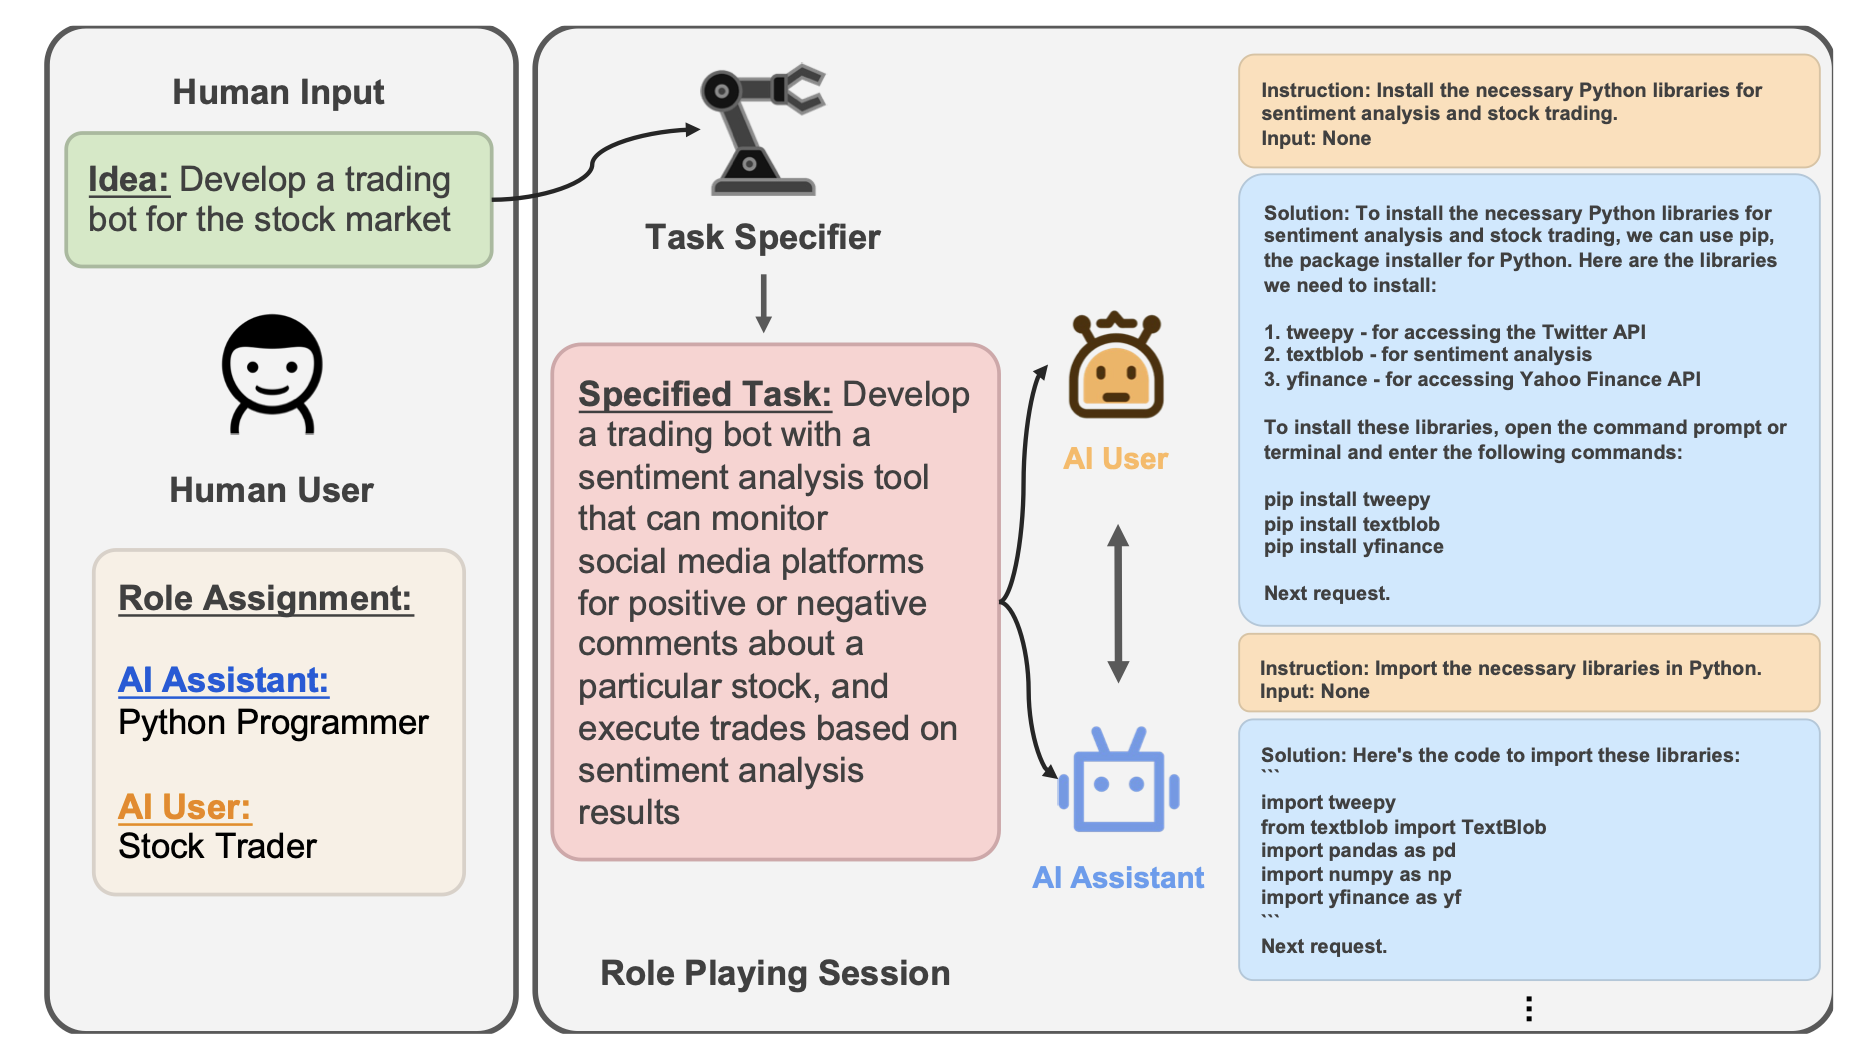
\includegraphics[width=1876pt]{figures/CAMEL.png}};
\fill[fill={rgb,255:red,243;green,243;blue,243}] (153,68) rectangle (418,118);
\node[anchor=center,inner sep=0pt,outer sep=0pt,align=center,text width=259pt,text=black,font={\fontsize{51.925}{59.1945}\selectfont\sffamily\bfseries}] at (285.5,93) {人类输入};
\fill[fill={rgb,255:red,213;green,231;blue,198}] (75,145) rectangle (482,255);
\node[anchor=center,inner sep=0pt,outer sep=0pt,align=center,text width=401pt,text=black,font={\fontsize{42.7125}{48.6922}\selectfont\sffamily}] at (278.5,200) {\textbf{构想：}开发一个\\股票市场交易机器人};
\fill[fill={rgb,255:red,243;green,243;blue,243}] (153,465) rectangle (423,516);
\node[anchor=center,inner sep=0pt,outer sep=0pt,align=center,text width=264pt,text=black,font={\fontsize{51.925}{59.1945}\selectfont\sffamily\bfseries}] at (288,490.5) {人类用户};
\fill[fill={rgb,255:red,248;green,239;blue,227}] (110,573) rectangle (446,626);
\node[anchor=center,inner sep=0pt,outer sep=0pt,align=center,text width=330pt,text=black,font={\fontsize{44.8062}{51.0791}\selectfont\sffamily\bfseries}] at (278,599.5) {角色分配：};
\fill[fill={rgb,255:red,248;green,239;blue,227}] (110,656) rectangle (447,700);
\node[anchor=center,inner sep=0pt,outer sep=0pt,align=left,text width=331pt,text={rgb,255:red,9;green,85;blue,230},font={\fontsize{44.8062}{51.0791}\selectfont\sffamily\bfseries}] at (278.5,678) {AI 助手：};
\fill[fill={rgb,255:red,248;green,239;blue,227}] (110,704) rectangle (447,754);
\node[anchor=center,inner sep=0pt,outer sep=0pt,align=left,text width=331pt,text=black,font={\fontsize{44.8062}{51.0791}\selectfont\sffamily}] at (278.5,729) {Python 程序员};
\fill[fill={rgb,255:red,248;green,239;blue,227}] (110,781) rectangle (447,824);
\node[anchor=center,inner sep=0pt,outer sep=0pt,align=left,text width=331pt,text={rgb,255:red,233;green,139;blue,0},font={\fontsize{44.8062}{51.0791}\selectfont\sffamily\bfseries}] at (278.5,802.5) {AI 用户：};
\fill[fill={rgb,255:red,248;green,239;blue,227}] (110,828) rectangle (447,876);
\node[anchor=center,inner sep=0pt,outer sep=0pt,align=left,text width=331pt,text=black,font={\fontsize{44.8062}{51.0791}\selectfont\sffamily}] at (278.5,852) {股票交易员};
\fill[fill={rgb,255:red,243;green,243;blue,243}] (630,211) rectangle (907,264);
\node[anchor=center,inner sep=0pt,outer sep=0pt,align=center,text width=271pt,text=black,font={\fontsize{51.5063}{58.7171}\selectfont\sffamily\bfseries}] at (768.5,237.5) {任务细化器};
\fill[fill={rgb,255:red,250;green,209;blue,207}] (573,365) rectangle (978,838);
\node[anchor=north west,inner sep=0pt,outer sep=0pt,align=left,text width=393pt,text=black,font={\fontsize{43.1313}{48.7383}\selectfont\sffamily}] at (578,370) {\textbf{具体任务：}开发一个带有情绪分析工具的交易机器人，监测社交媒体平台上关于某只股票的正面或负面评论，并根据情绪分析结果执行交易。};
\fill[fill={rgb,255:red,243;green,243;blue,243}] (1033,439) rectangle (1212,479);
\node[anchor=center,inner sep=0pt,outer sep=0pt,align=center,text width=173pt,text={rgb,255:red,252;green,179;blue,79},font={\fontsize{43.55}{49.647}\selectfont\sffamily\bfseries}] at (1122.5,459) {AI 用户};
\fill[fill={rgb,255:red,243;green,243;blue,243}] (1024,864) rectangle (1217,911);
\node[anchor=center,inner sep=0pt,outer sep=0pt,align=center,text width=187pt,text={rgb,255:red,96;green,153;blue,239},font={\fontsize{43.55}{49.647}\selectfont\sffamily\bfseries}] at (1120.5,887.5) {AI 助手};
\fill[fill={rgb,255:red,243;green,243;blue,243}] (590,948) rectangle (985,1002);
\node[anchor=center,inner sep=0pt,outer sep=0pt,align=center,text width=389pt,text=black,font={\fontsize{49.4125}{56.3303}\selectfont\sffamily\bfseries}] at (787.5,975) {角色扮演会话};
\fill[fill={rgb,255:red,243;green,243;blue,243}] (531,1008) rectangle (1840,1260);
\draw[draw=black!65,line width=5pt,rounded corners=40pt] (534,28) rectangle (1834,1255);
\fill[fill={rgb,255:red,243;green,243;blue,243}] (1236,51) rectangle (1825,1234);
\draw[fill={rgb,255:red,255;green,224;blue,183},draw={rgb,255:red,214;green,192;blue,159},line width=2pt,rounded corners=18pt] (1239,55) rectangle (1820,183);
\node[anchor=north west,inner sep=0pt,outer sep=0pt,align=left,text width=536pt,text=black,font={\fontsize{34.7563}{39.2746}\selectfont\sffamily}] at (1260,70) {\textbf{指令：}安装情绪分析与股票交易所需的 Python 库。\\\textbf{输入：}无};
\draw[fill={rgb,255:red,202;green,231;blue,250},draw={rgb,255:red,174;green,203;blue,220},line width=2pt,rounded corners=18pt] (1239,192) rectangle (1820,716);
\node[anchor=north west,inner sep=0pt,outer sep=0pt,align=left,text width=536pt,text=black,font={\fontsize{32.6625}{36.9086}\selectfont\sffamily}] at (1260,208) {\textbf{解决方案：}可用 Python 的软件包安装器 pip，安装情绪分析和股票交易所需的库。需要安装：\\1. tweepy：访问 Twitter API\\2. textblob：情绪分析\\3. yfinance：访问 Yahoo Finance API\\[0.2em]请打开命令提示符或终端，输入以下命令：\\\texttt{pip install tweepy}\\\texttt{pip install textblob}\\\texttt{pip install yfinance}\\[0.2em]下一项请求。};
\draw[fill={rgb,255:red,255;green,224;blue,183},draw={rgb,255:red,214;green,192;blue,159},line width=2pt,rounded corners=18pt] (1239,725) rectangle (1820,818);
\node[anchor=north west,inner sep=0pt,outer sep=0pt,align=left,text width=536pt,text=black,font={\fontsize{34.7563}{39.2746}\selectfont\sffamily}] at (1260,739) {\textbf{指令：}在 Python 中导入所需的库。\\\textbf{输入：}无};
\draw[fill={rgb,255:red,202;green,231;blue,250},draw={rgb,255:red,174;green,203;blue,220},line width=2pt,rounded corners=18pt] (1239,827) rectangle (1820,1215);
\node[anchor=north west,inner sep=0pt,outer sep=0pt,align=left,text width=536pt,text=black,font={\fontsize{33.5}{37.855}\selectfont\sffamily}] at (1260,842) {\textbf{解决方案：}以下代码用于导入这些库：\\\texttt{```}\\\texttt{import tweepy}\\\texttt{from textblob import TextBlob}\\\texttt{import pandas as pd}\\\texttt{import numpy as np}\\\texttt{import yfinance as yf}\\\texttt{```}\\下一项请求。};
\node[anchor=north west,inner sep=0pt,outer sep=0pt,align=left,text width=50pt,text=black,font={\fontsize{41.875}{47.3187}\selectfont\sffamily}] at (1510,1223) {$\vdots$};
\pgfresetboundingbox
\path[use as bounding box] (0,0) rectangle (1876,1270);
\end{tikzpicture}}
\endgroup
